\documentclass{standalone}
\usepackage{tikz}
\usetikzlibrary{decorations.pathreplacing,decorations.pathmorphing}
\usetikzlibrary{fit,quotes}
\usepackage{yquant, braket}
\newcommand{\spring}[3][0mm]{
  % optional arg 1: vertical shift amount
  % arg 2: box label in which to place spring
  % arg 3: height of spring
  \def \shiftamount {#1}
  \draw[decoration={aspect=0.1, segment length=1.5mm, amplitude=#3, coil},decorate] ([yshift=-\shiftamount] #2.west) -- ([yshift=-\shiftamount] #2.east) ;
  \draw [dashed] (#2.north west) -- (#2.south west);
  \draw [dashed] (#2.north east) -- (#2.south east);
}


\begin{document}
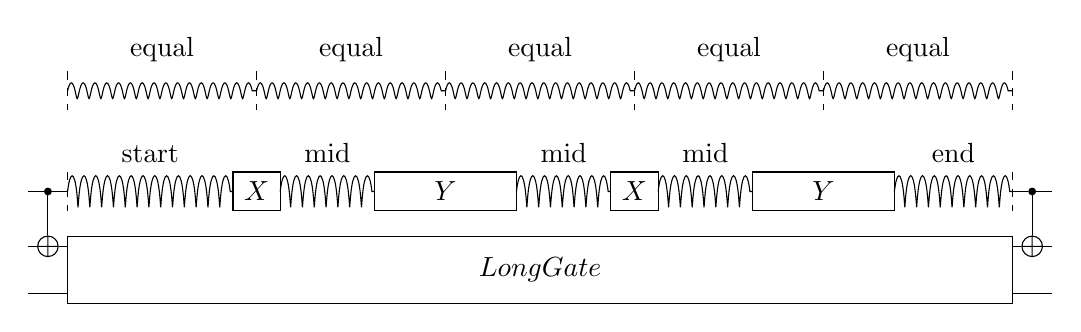
\begin{tikzpicture}
  \def \xlen {3mm}
  \def \ylen {9mm}
  \def \eqlen {12mm}
  \newlength{\startlen}
  \newlength{\midlen}
  \newlength{\termlen}
  \newlength{\longlen}
  \setlength{\startlen}{\dimexpr(\eqlen-\xlen/2)\relax}
  \setlength{\midlen}{\dimexpr(\eqlen-\xlen/2-\ylen/2)\relax}
  \setlength{\termlen}{\dimexpr(\eqlen-\ylen/2)\relax}
  \setlength{\longlen}{\dimexpr(\eqlen*5)\relax}
  \begin{yquant*}[operator/separation=0mm, register/separation=3mm]
    nobit p;
    qubit {} q[3];
    hspace {5mm} p;
    ["equal", name=eq0, x radius=\eqlen, draw=none] box {} p;
    ["equal", name=eq1, x radius=\eqlen, draw=none] box {} p;
    ["equal", name=eq2, x radius=\eqlen, draw=none] box {} p;
    ["equal", name=eq3, x radius=\eqlen, draw=none] box {} p;
    ["equal", name=eq4, x radius=\eqlen, draw=none] box {} p;
    cnot q[1] | q[0];
    ["start", name=ss, x radius=\startlen, draw=none] box {} q[0];
    [x radius=\xlen] box {$X$} q[0];
    ["mid", name=ms0, x radius=\midlen, draw=none] box {} q[0];
    [x radius=\ylen] box {$Y$} q[0];
    ["mid", name=ms1, x radius=\midlen, draw=none] box {} q[0];
    [x radius=\xlen] box {$X$} q[0];
    ["mid", name=ms2, x radius=\midlen, draw=none] box {} q[0];
    [x radius=\ylen] box {$Y$} q[0];
    ["end", name=es, x radius=\termlen, draw=none] box {} q[0];
    [x radius=\longlen] box {$LongGate$} (q[1], q[2]);
    cnot q[1] | q[0];
  \end{yquant*}
  \spring{eq0}{1mm}
  \spring{eq1}{1mm}
  \spring{eq2}{1mm}
  \spring{eq3}{1mm}
  \spring{eq4}{1mm}
  \spring{ss}{2mm}
  \spring{ms0}{2mm}
  \spring{ms1}{2mm}
  \spring{ms2}{2mm}
  \spring{es}{2mm}
\end{tikzpicture}
\end{document}